One of the main improvements brought in the analysis is the usage of a new multivariate discriminant for electron selection in all data taking periods.

Reconstructed electrons are now identified and isolated by means of an e\textbf{X}treme \textbf{G}radient \textbf{Boost}ing (XGBoost) optimized distributed
gradient boosting library designed to be highly efficient, flexible and portable. It implements machine learning algorithms under the Gradient Boosting framework
and exploits observables from the electromagnetic cluster, the matching between the cluster and the electron track, observables based exclusively on tracking
measurements as well as particle flow isolation sums. The full list of used features can be found in the Table~\ref{tab:ele_ID_input_variables}.

\begin{table}[H]
\scriptsize
   \centering
   \begin{tabular}{c|l}
\hline
\hline
Observable type & Observable name \\
\hline
\multirow{6}{*}{Cluster shape}
	& RMS of the energy-crystal number spectrum along $\eta$ and $\varphi$; $\sigma_{i\eta i\eta}$, $\sigma_{i\varphi i\varphi}$ \\
	& Super cluster width along $\eta$ and $\phi$ \\
	& Ratio of the hadronic energy behind the electron supercluster to the supercluster energy, $H/E$ \\
	& Circularity $(E_{5\times5} - E_{5\times1})/E_{5\times5}$ \\
	& Sum of the seed and adjacent crystal over the super cluster energy $R_{9}$ \\
	& For endcap traing bins: energy fraction in pre-shower $E_\text{PS}/E_\text{raw}$ \\
\hline
\multirow{2}{*}{Track-cluster matching}
	& Energy-momentum agreement $E_{tot}/p_{in}$, $E_{ele}/p_{out}$, $1/E_{tot} - 1/p_{in}$ \\
	& Position matching $\Delta\eta_{in}$, $\Delta\varphi_{in}$, $\Delta\eta_{seed}$ \\
\hline
\multirow{5}{*}{tracking}
   & Fractional momentum loss $f_{brem} = 1 - p_{out}/p_{in}$ \\
   & Number of hits of the KF and GSF track $N_{KF}$, $N_{GSF}$ \\ %$(\mathord{\cdot})$ \\
   & Reduced $\chi^2$ of the KF and GSF track $\chi^{2}_{KF}$, $\chi^{2}_{\textrm{GSF}}$ \\
   & Number of expected but missing inner hits \\ %$(\mathord{\cdot})$ \\
   & Probability transform of conversion vertex fit $\chi^2$ \\ % $(\mathord{\cdot})$ \\
\hline
\multirow{3}{*}{isolation}
   & Particle Flow photon isolation sum \\ %$(\mathord{\cdot})$ \\
   & Particle Flow charged hadrons isolation sum \\ %$(\mathord{\cdot})$ \\
   & Particle Flow neutral hadrons isolation sum \\ %$(\mathord{\cdot})$ \\
\hline
\multirow{1}{*}{For PU-resilience}
   & Mean energy density in the event: $\rho$ \\ %$(\mathord{\cdot})$ \\
\hline
\hline
     \end{tabular}
\small
    \caption{Overview of input features to the identification classifier.} %Variables not used in the Run 2 MVA are marked with  $(\mathord{\cdot})$.}
    \label{tab:ele_ID_input_variables}
\end{table}


The model is trained on 2016, 2017, and 2018 Drell-Yan with jets MC sample for both signal and background. The separate training for three periods guarantees
optimal performance during the whole Run 2 data taking period. The simulated samples used to train the model are listed bellow.

\begin{itemize}
\item \textbf{2016} \begin{verbatim}/DYJetsToLL_M-50_TuneCUETP8M1_13TeV-amcatnloFXFX-pythia8/RunIISummer16MiniAODv2-PUMoriond17_80X_mcRun2_asymptotic_2016_TrancheIV_v6_ext2-v1/MINIAODSIM\end{verbatim}
\item \textbf{2017} \begin{verbatim}/DYJetsToLL_M-50_TuneCP5_13TeV-madgraphMLM-pythia8/RunIIFall17MiniAOD-RECOSIMstep_94X_mc2017_realistic_v10-v1/MINIAODSIM\end{verbatim}
\item \textbf{2018} \begin{verbatim}/DYJetsToLL_M-50_TuneCP5_13TeV-madgraphMLM-pythia8/RunIIAutumn18MiniAOD-102X_upgrade2018_realistic_v15-v1/MINIAODSIM\end{verbatim}
\end{itemize}

Several studies have been conducted on 2016 Drell-Yan with jets MC sample. The XGBoost framework was first used in 2017 and the model was trained on 2017
Drell-Yan with jets MC sample. This model is known as 2017 ID+ISO V2. The same framework was then used to train the model on 2016 MC (2016 ID+ISO) and finally
on 2018 MC (2018 ID+ISO). In Fig.~\ref{fig:ele_ID_ISO_ROC_2016} one can see the ROC curves obtained using 2016 Drell-Yan with jets MC sample. As expected, the
model trained on 2016 MC using electron identification and isolation features outperforms the model trained on 2016 MC using only identification features and
the model obtained after applying 2017 ID+ISO V2 training on 2016 Drell-Yan with jets MC sample.

In Fig.~\ref{fig:ele_ID_ISO_ROC_2016_} one can see the ROC curve for the model trained on 2016 MC using electron identification and isolation features and ROC
curve when applying sequential approach meaning applying isolation cut after cutting on the distribution obtained by training using only identification features.
As expected, the model obtained using electron identification and isolation features outperforms the sequential approach model.

\begin{figure}[!htb]
   \vspace*{0.3cm}
   \begin{center}
      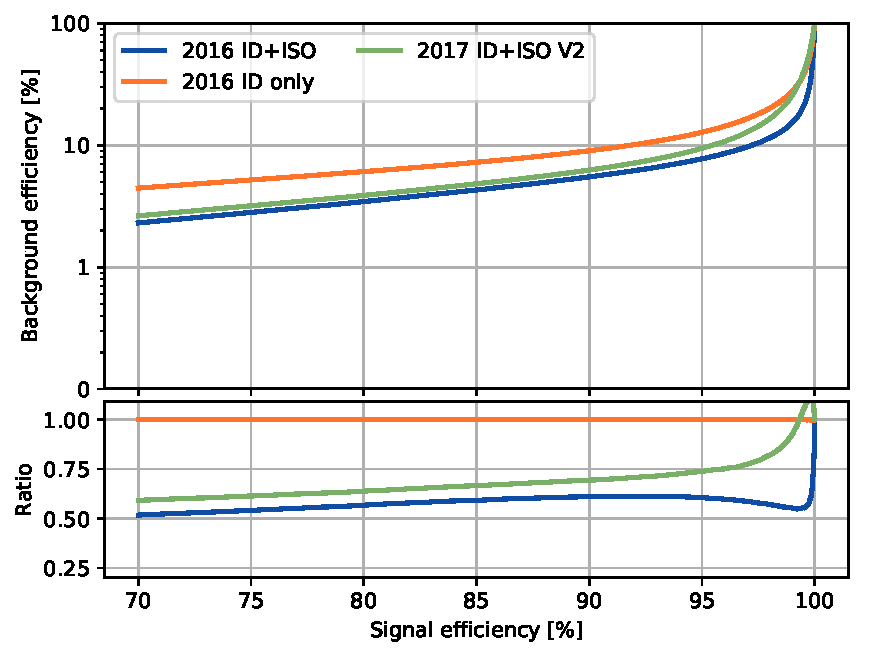
\includegraphics[width=0.45\textwidth]{Figures/Electrons/2016_EB1_5.pdf}
      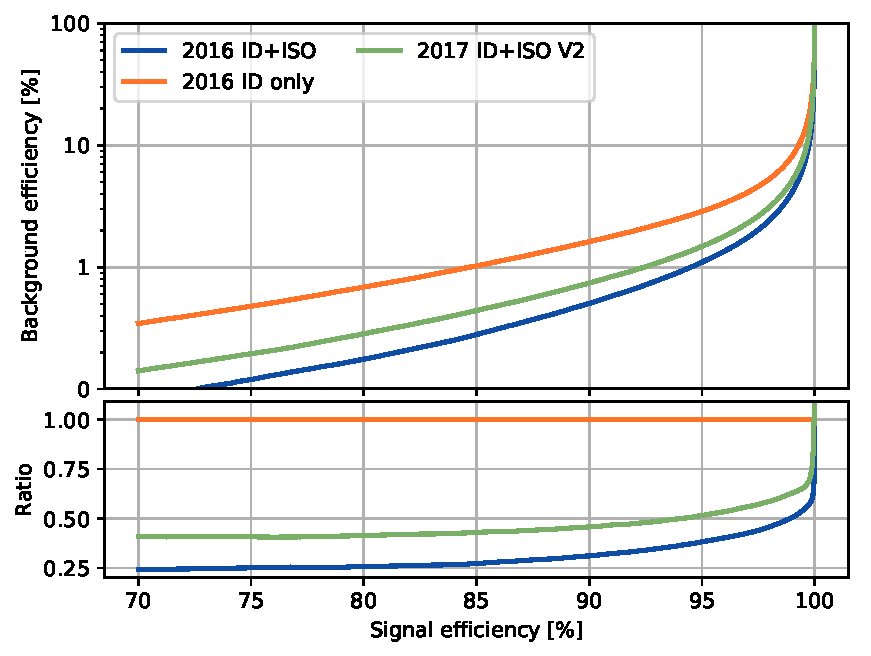
\includegraphics[width=0.45\textwidth]{Figures/Electrons/2016_EB1_10.pdf} \\
      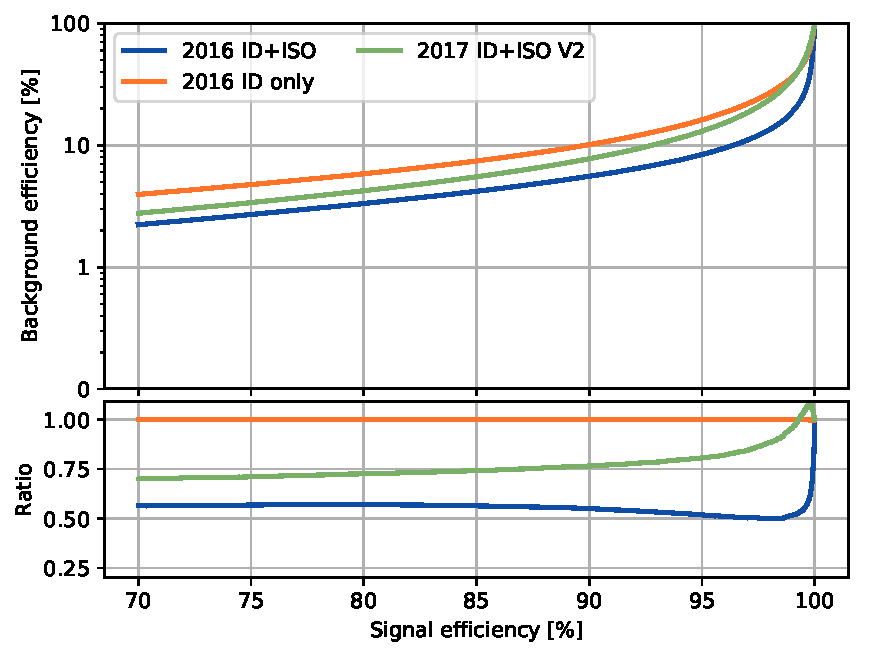
\includegraphics[width=0.45\textwidth]{Figures/Electrons/2016_EB2_5.pdf}
      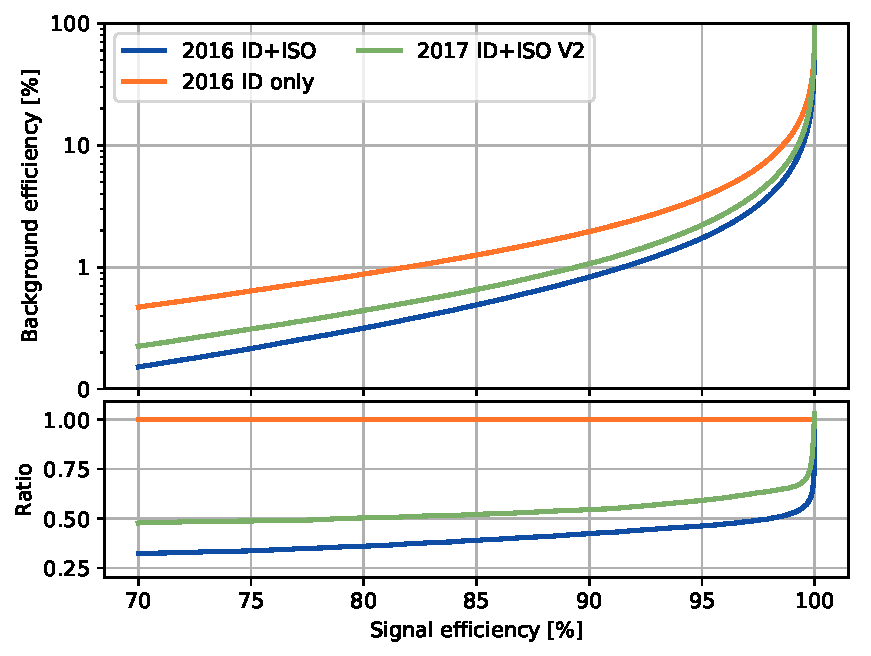
\includegraphics[width=0.45\textwidth]{Figures/Electrons/2016_EB2_10.pdf} \\
      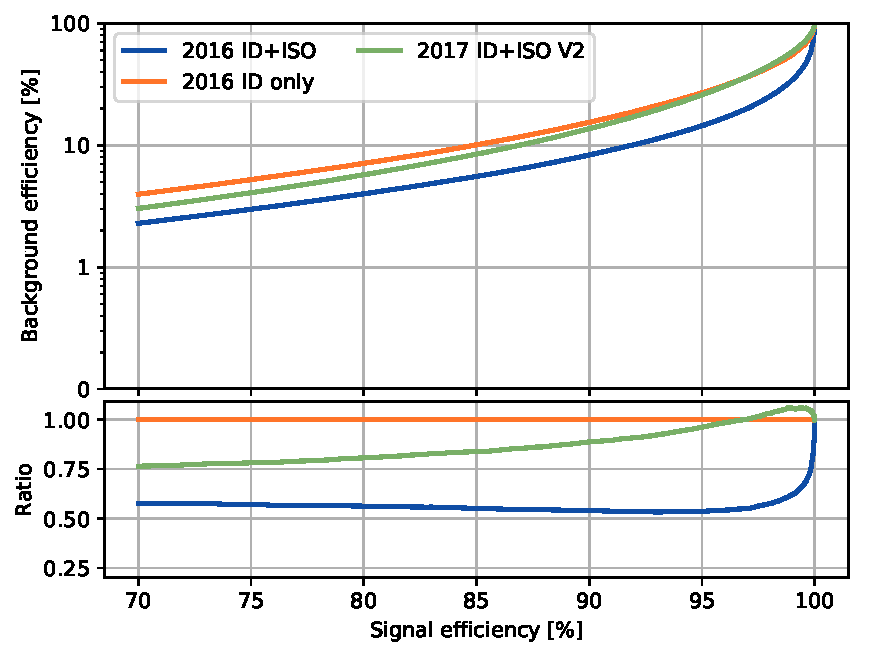
\includegraphics[width=0.45\textwidth]{Figures/Electrons/2016_EE_5.pdf}
      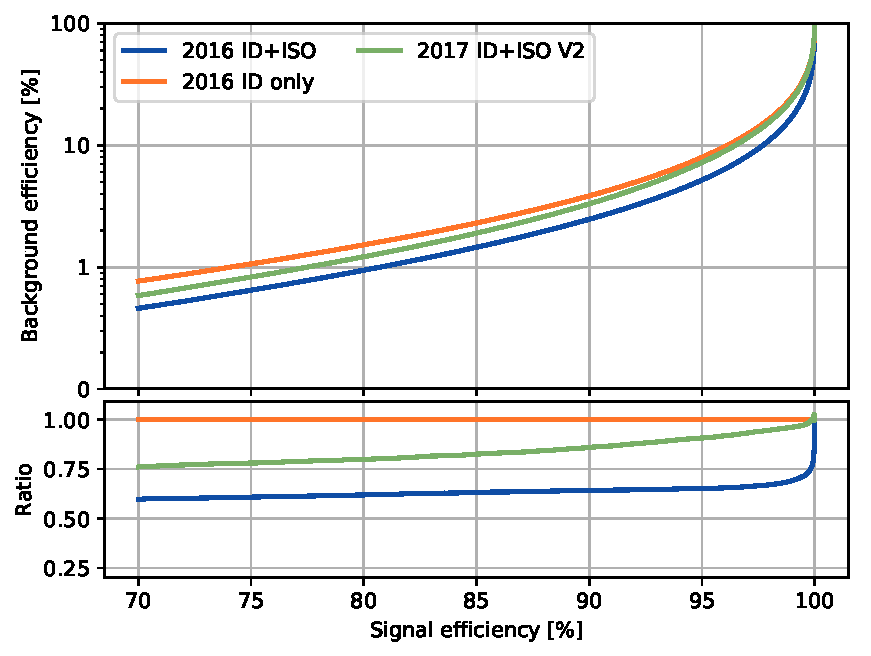
\includegraphics[width=0.45\textwidth]{Figures/Electrons/2016_EE_10.pdf} \\
   \caption{The receiver operating characteristic curves, representing the background efficiency vs signal efficiency, of the MVA trained on 2016 Drell-Yan with
   jets MC sample. Performance are shown for electrons with $5 < p_T < 10 $ GeV (left), $p_T > 10$ GeV (right), and $|\eta| < 0.8$ (top),
   $0.8 < |\eta| < 1.479$ (middle), and $|\eta| > 1.479$ (bottom).
   \label{fig:ele_ID_ISO_ROC_2016}}
   \end{center}
\end{figure}


\begin{figure}[!htb]
   \vspace*{0.3cm}
   \begin{center}
      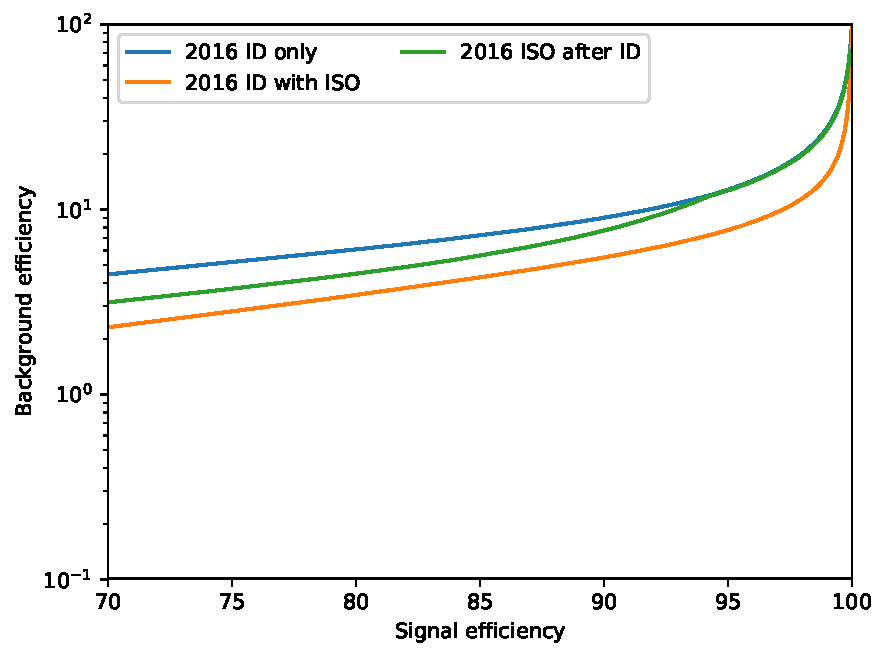
\includegraphics[width=0.45\textwidth]{Figures/Electrons/2016_EB1_5_.pdf}
      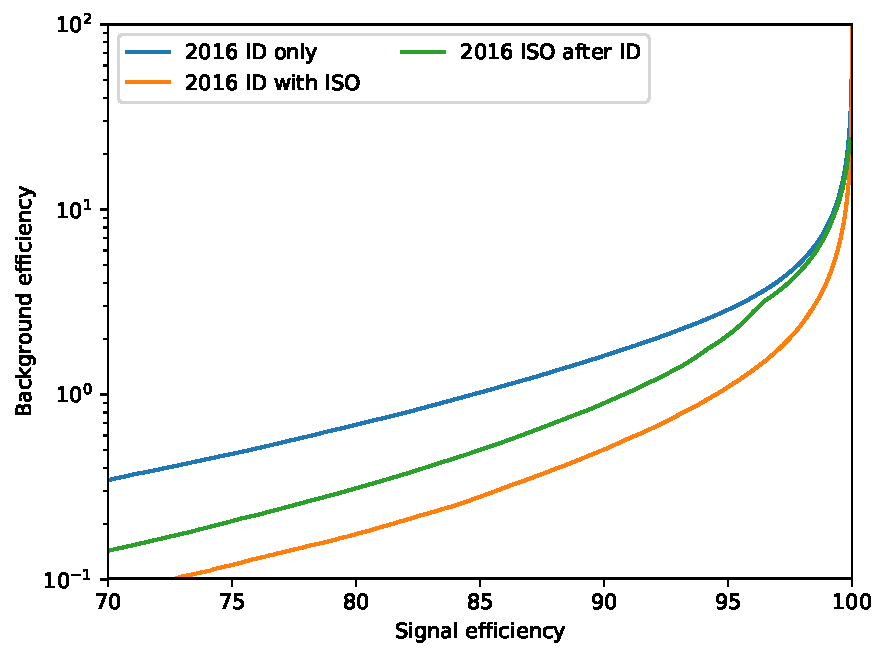
\includegraphics[width=0.45\textwidth]{Figures/Electrons/2016_EB1_10_.pdf} \\
      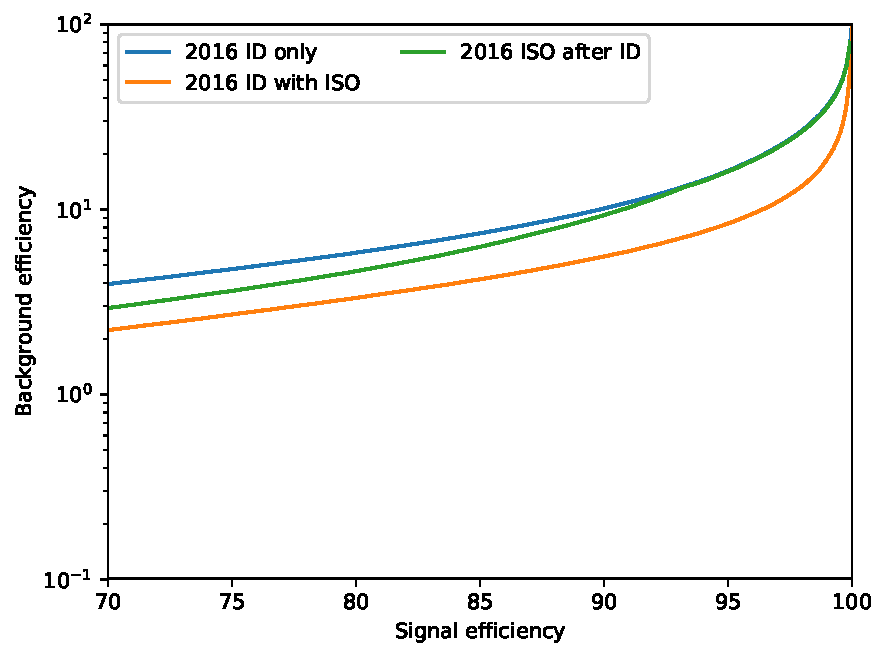
\includegraphics[width=0.45\textwidth]{Figures/Electrons/2016_EB2_5_.pdf}
      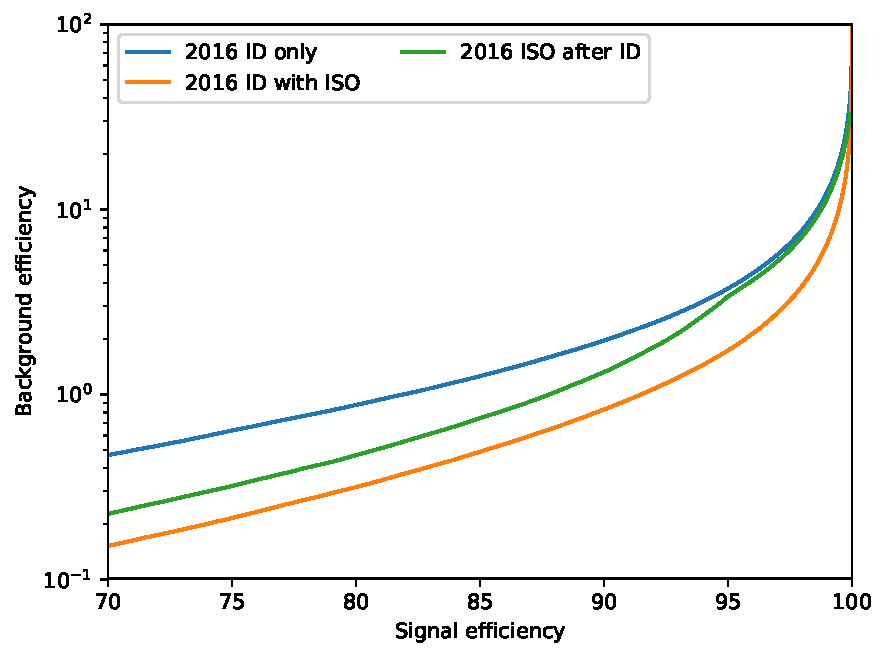
\includegraphics[width=0.45\textwidth]{Figures/Electrons/2016_EB2_10_.pdf} \\
      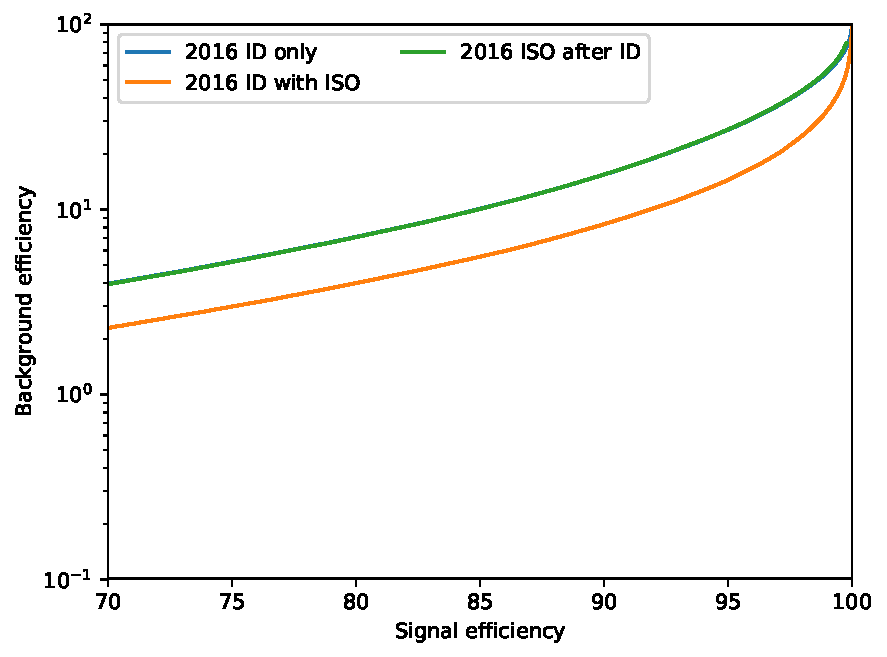
\includegraphics[width=0.45\textwidth]{Figures/Electrons/2016_EE_5_.pdf}
      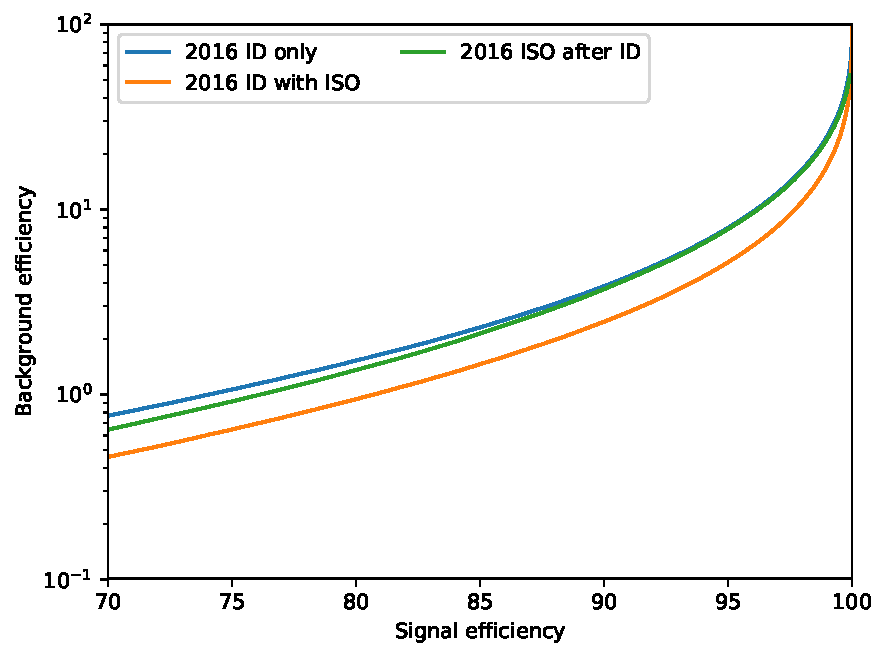
\includegraphics[width=0.45\textwidth]{Figures/Electrons/2016_EE_10_.pdf} \\
   \caption{The receiver operating characteristic curves, representing the background efficiency vs signal efficiency, of the MVA trained on 2016 Drell-Yan with
   jets MC sample. Performance are shown for electrons with $5 < p_T < 10 $ GeV (left), $p_T > 10$ GeV (right), and $|\eta| < 0.8$ (top),
   $0.8 < |\eta| < 1.479$ (middle), and $|\eta| > 1.479$ (bottom).
   \label{fig:ele_ID_ISO_ROC_2016_}}
   \end{center}
\end{figure}

The Fig.~\ref{fig:ele_MVA_score_2018} shows output of the multiclassifier discriminant i.e. MVA score for prompt electrons from Drell-Yan events and
misidentified electrons originating from jets in Drell-Yan events. The performance of  model trained on 2018 MC using electron identification and isolation
features outperforms the model obtained after applying 2017 ID+ISO V2 training on 2018 Drell-Yan with jets MC sample as shown in Fig.~\ref{fig:ele_ID_ISO_ROC_2018}.

\begin{figure}[!htb]
   \vspace*{0.3cm}
   \begin{center}
      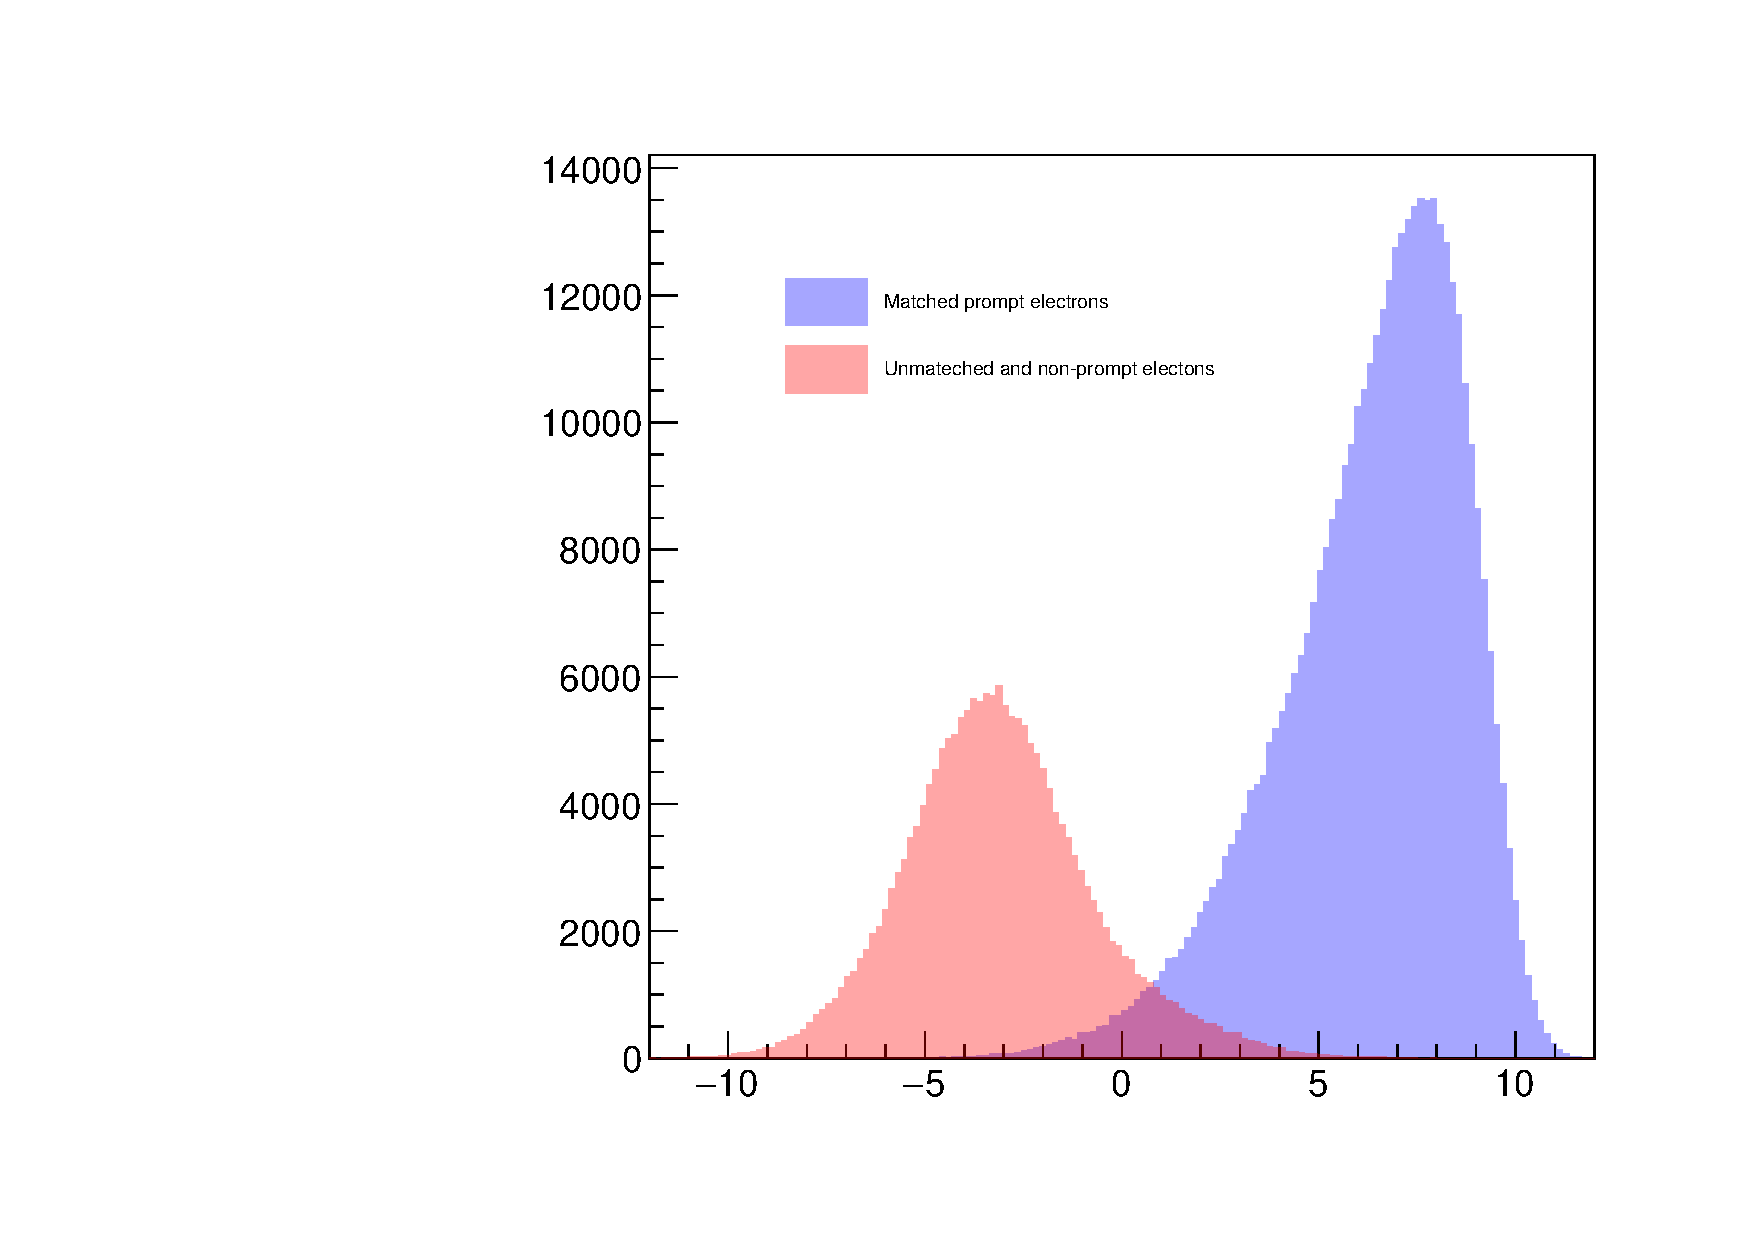
\includegraphics[width=0.80\textwidth]{Figures/Electrons/Ele_BDTv2_Score.pdf}
      \caption{The Output of the multiclassifier discriminant for prompt electrons matched to truth electrons from $Z$ decay (blue) and for misindentified
      electrons (red). Events are all taken from Drell-Yan with jets MC sample.
      \label{fig:ele_MVA_score_2018}}
   \end{center}
\end{figure}

\begin{figure}[!htb]
   \vspace*{0.3cm}
   \begin{center}
      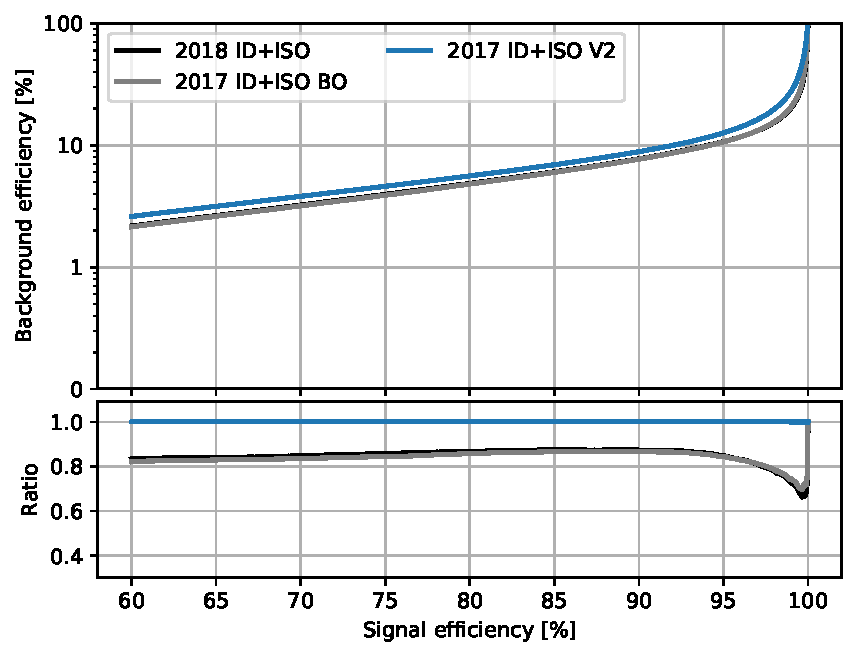
\includegraphics[width=0.45\textwidth]{Figures/Electrons/2018_EB1_5.pdf}
      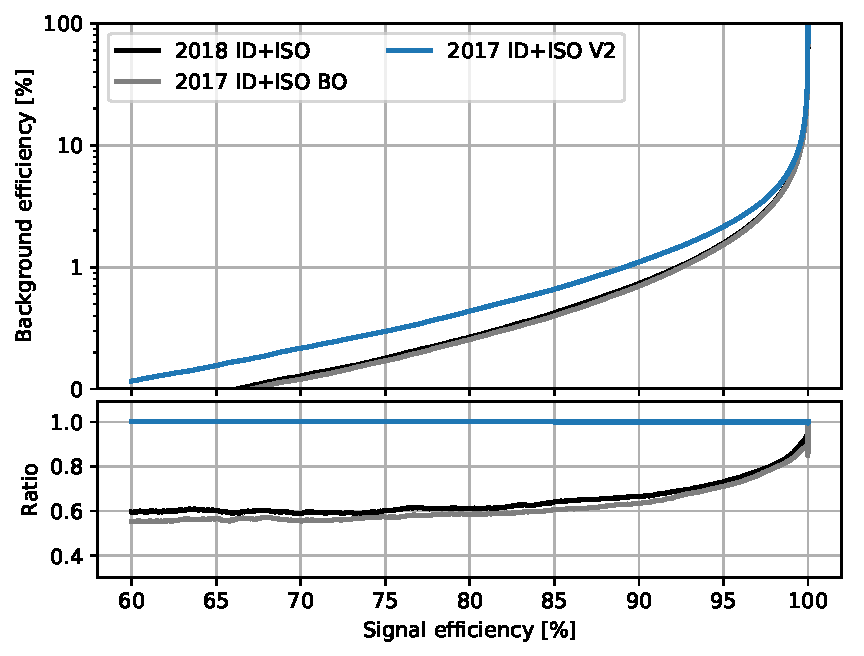
\includegraphics[width=0.45\textwidth]{Figures/Electrons/2018_EB1_10.pdf} \\
      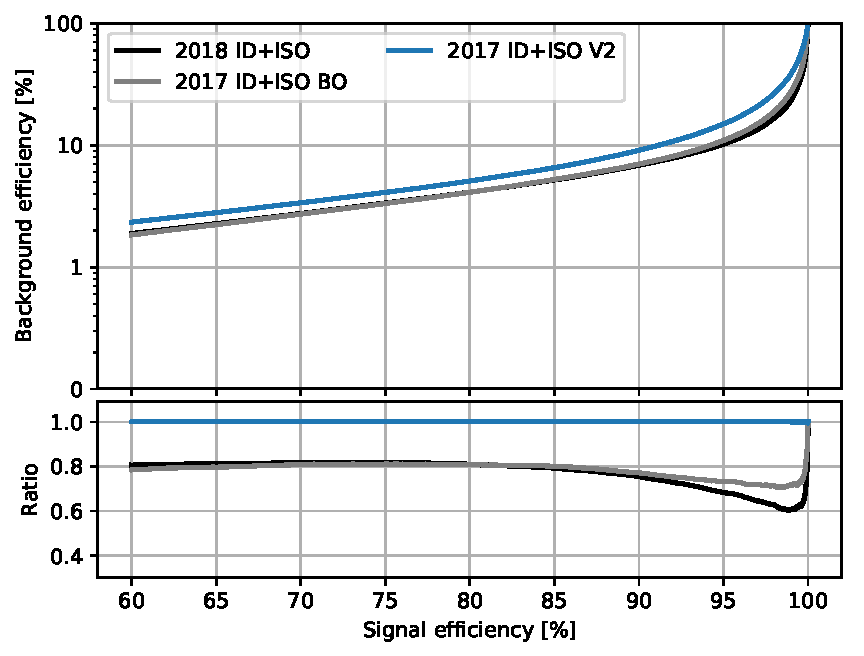
\includegraphics[width=0.45\textwidth]{Figures/Electrons/2018_EB2_5.pdf}
      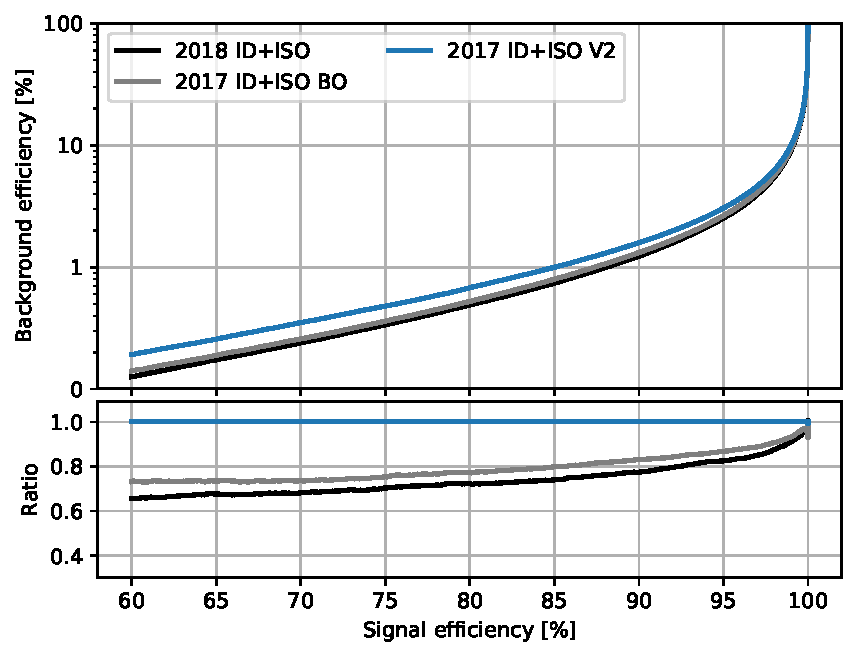
\includegraphics[width=0.45\textwidth]{Figures/Electrons/2018_EB2_10.pdf}\\
      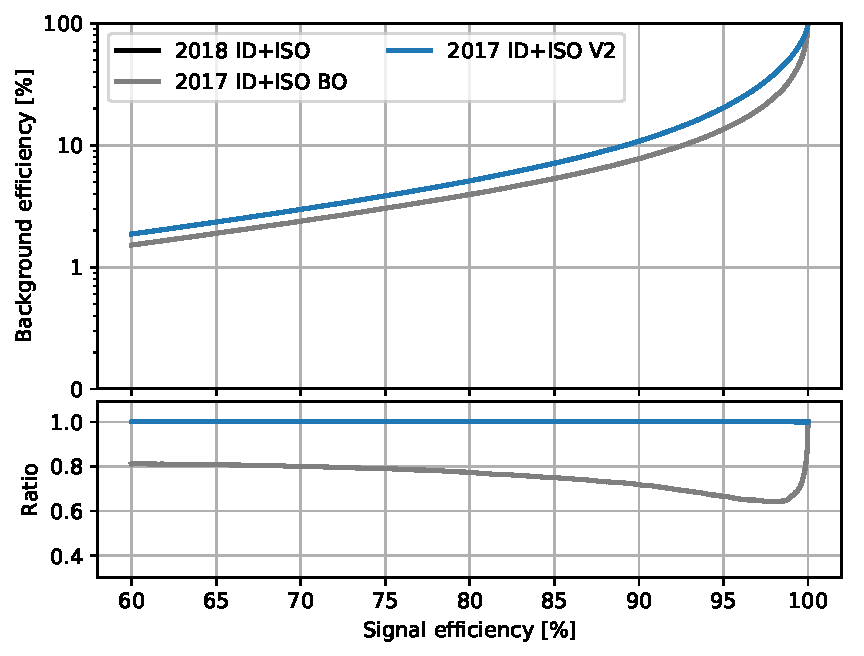
\includegraphics[width=0.45\textwidth]{Figures/Electrons/2018_EE_5.pdf}
      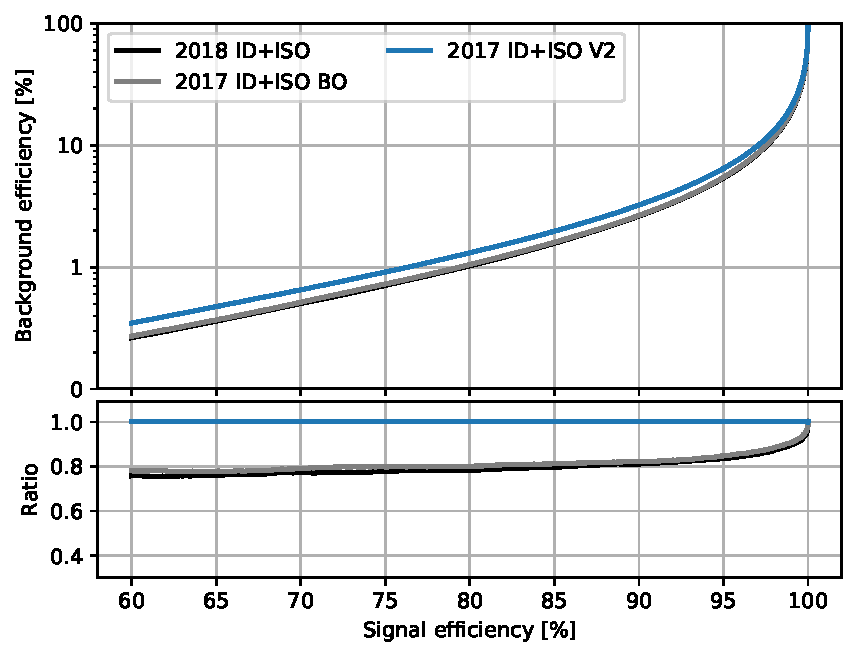
\includegraphics[width=0.45\textwidth]{Figures/Electrons/2018_EE_10.pdf} \\
   \caption{The receiver operating characteristic curves, representing the background efficiency vs signal efficiency, of the MVA trained on the 2017 Drell-Yan
   with jets MC sample and applied on the 2018 Drell-Yan with jets MC sample. The training combines identification and isolation fautures. Performance are shown
   for electrons with $5 < p_T < 10$ GeV (left), $p_T > 10 GeV$ (right), and $|\eta|<0.8$ (top), $0.8 < |\eta| < 1.479$ (middle), and $|\eta| > 1.479$ (bottom).
   V1 and V2 versions of training are compared, exploiting TMVA and xgboost training libraries respectively.
   \label{fig:ele_ID_ISO_ROC_2018}}
   \end{center}
\end{figure}

The impact of the transition from the TMVA (V1) to the XGBoost(V2) training framework is shown in Fig.~\ref{fig:ele_ID_ISO_ROC_V1_vs_V2}, showing a noticeable improvement.
% The working points shown are chosen so as to get the  same signal efficiency as a cut on MVA ID and a cut on the PF isolation, in each $p_T$ and $\eta$ bin.

\begin{figure}[!htb]
   \vspace*{0.3cm}
   \begin{center}
      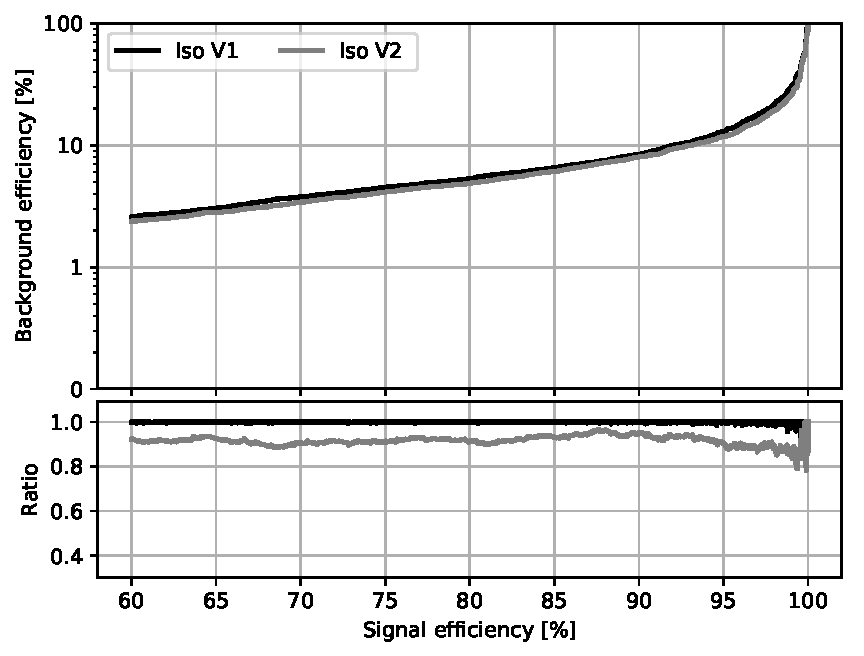
\includegraphics[width=0.45\textwidth]{Figures/Electrons/2018_EB1_5_.pdf}
      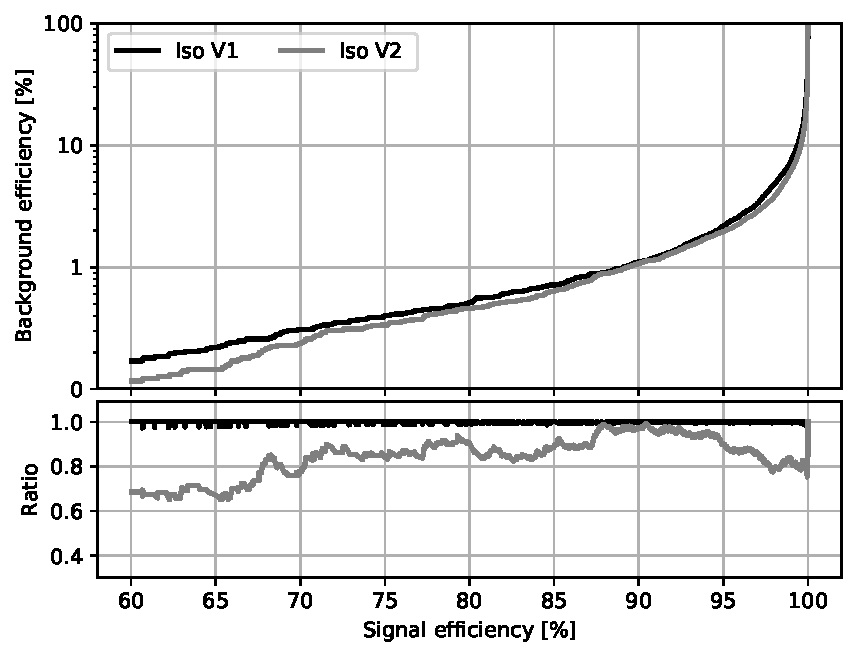
\includegraphics[width=0.45\textwidth]{Figures/Electrons/2018_EB1_10_.pdf} \\
      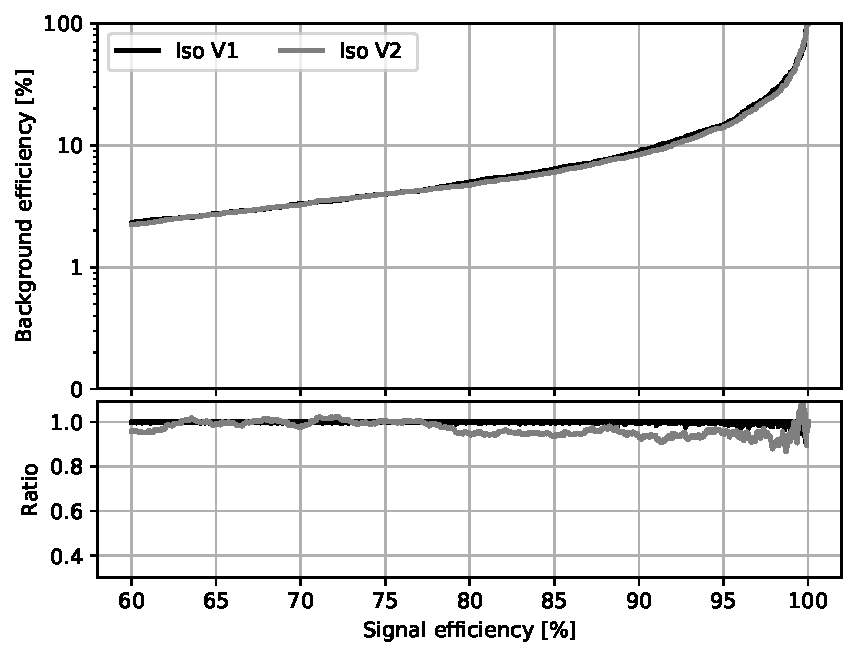
\includegraphics[width=0.45\textwidth]{Figures/Electrons/2018_EB2_5_.pdf}
      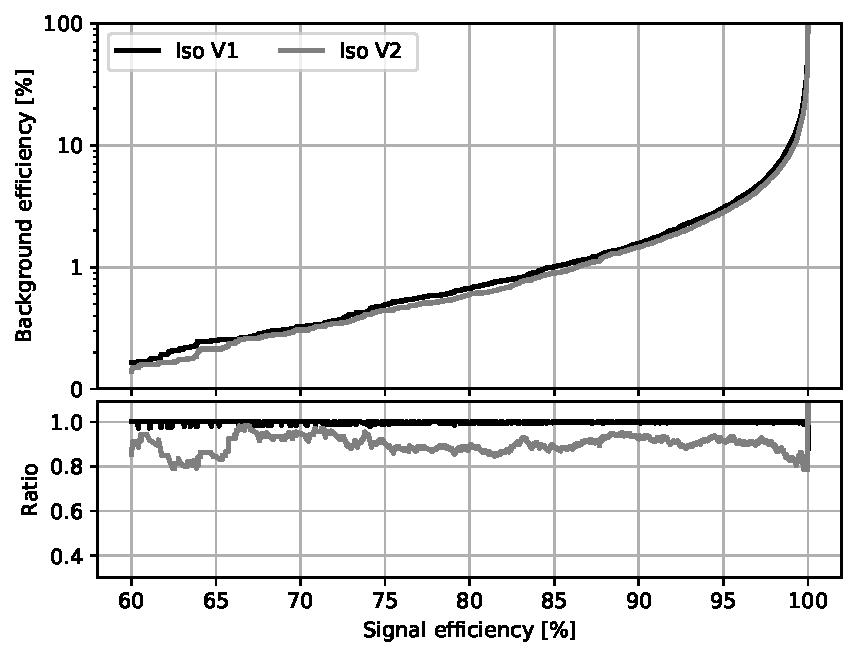
\includegraphics[width=0.45\textwidth]{Figures/Electrons/2018_EB2_10_.pdf} \\
      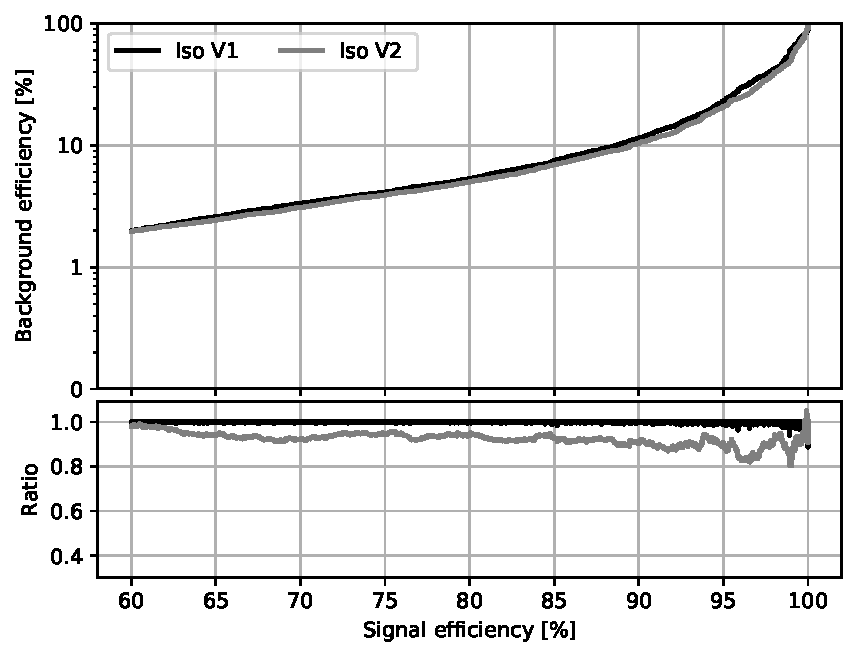
\includegraphics[width=0.45\textwidth]{Figures/Electrons/2018_EE_5_.pdf}
      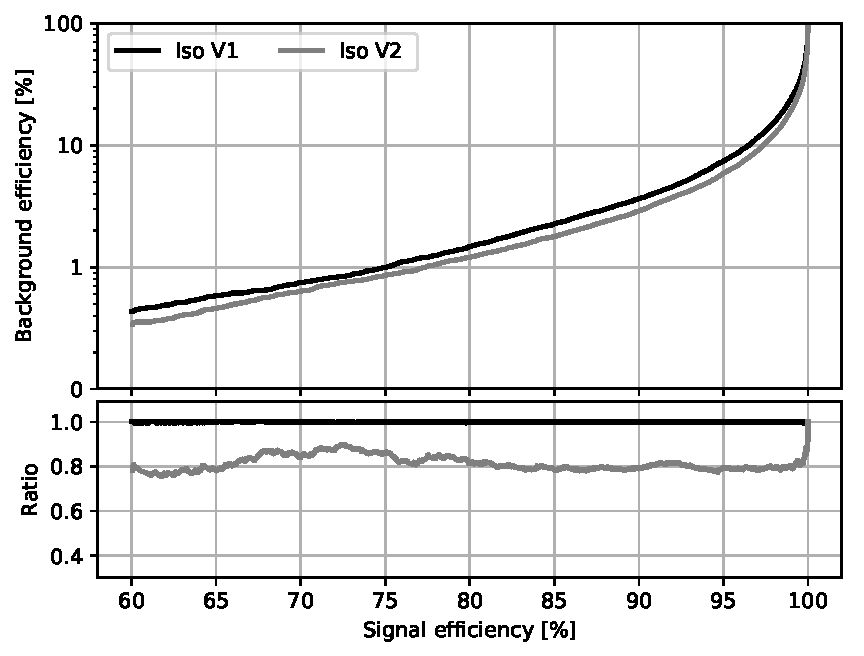
\includegraphics[width=0.45\textwidth]{Figures/Electrons/2018_EE_10_.pdf} \\
   \caption{Performance comparison, background efficiency vs signal efficiency, of the MVA trained using TMVA framework (V1) and XGBoost framework (V2). The
   performance are shown for electrons with $5 < p_T < 10$ GeV (left), $p_T > 10 GeV$ (right), and $|\eta|<0.8$ (top), $0.8 < |\eta| < 1.479$ (middle), and
   $|\eta| > 1.479$ (bottom).
\label{fig:ele_ID_ISO_ROC_V1_vs_V2}}
\end{center}
\end{figure}



% \begin{figure}[!htb]
% \vspace*{0.3cm}
% \begin{center}
% \includegraphics[width=0.5\textwidth]{Figures/Electrons/ele_overtraining.png}
% \caption{BDT output for the training and testing sample for true and fake electrons in the high-$p_T$ endcap training bins.
% \label{fig:ele_ID_BDT_output}}
% \end{center}
% \end{figure}

%Table~\ref{tab:ele_ID_input_variables} summarizes the full list of observables used as input to the classifier
Tables~\ref{tab:ele_ID_WPA},~\ref{tab:ele_ID_WPB} and ~\ref{tab:ele_ID_WPC} list the cuts values applied to the MVA output for 2016, 2017, 2018 training, respectively. For 2018, the corresponding signal and background efficiencies are given as examples.They are very similar for 2016 and 2017. 
%e for the chosen working point. 
For the analysis, loose electrons have to pass this MVA identification and isolation working point.

\begin{table}[h!]
%\scriptsize
    \centering
    \begin{tabular}{c|c c c}
\hline
\multicolumn{4}{|c|}{2016 Datasets}                                                                 \\
\hline %----------------------------------------------------------------------------------------
minimum BDT score    &  $|\eta| < 0.8 $ & $0.8 < |\eta| < 1.479$ 	& $|\eta| > 1.479$      \\
\hline %----------------------------------------------------------------------------------------
$ 5 < p_T < 10 $ GeV &  0.9503      & 0.9461  	& 0.9387		\\
$p_T > 10$ GeV         &  0.3782	& 0.3587		&  -0.5745	\\
\hline %----------------------------------------------------------------------------------------
\hline %----------------------------------------------------------------------------------------
     \end{tabular}
\small
    \caption{Minimum BDT score required for passing the electron identification, for 2016 samples.}% \textbf{FIXME: WP to be defined!}}
    \label{tab:ele_ID_WPA}
\end{table}

\begin{table}[h!]
%\scriptsize
    \centering
    \begin{tabular}{c|c c c}
\hline
\multicolumn{4}{|c|}{2017 Datasets}                                                                 \\
\hline %----------------------------------------------------------------------------------------
minimum BDT score    &  $|\eta| < 0.8 $ & $0.8 < |\eta| < 1.479$ 	& $|\eta| > 1.479$      \\
\hline %----------------------------------------------------------------------------------------
$ 5 < p_T < 10 $ GeV &  0.8521    & 0.8268  	& 0.8694		\\
$p_T > 10$ GeV         &  0.9825    & 0.9692	& 0.7935	\\
\hline %----------------------------------------------------------------------------------------
\hline %----------------------------------------------------------------------------------------
     \end{tabular}
\small
    \caption{Minimum BDT score required for passing the electron identification, for 2017 samples.}% \textbf{FIXME: WP to be defined!}}
    \label{tab:ele_ID_WPB}
\end{table}

%2016
 %= (pt<=10 && ((fSCeta<0.8                  && BDT >  0.95034841889) ||
 %                                 (fSCeta>=0.8 && fSCeta<1.479 && BDT >  0.94606270058) ||
 %                                (fSCeta>=1.479               && BDT >  0.93872558098)))
 %                   || (pt>10  && ((fSCeta<0.8                  && BDT >  0.3782357877) ||
   %                                (fSCeta>=0.8 && fSCeta<1.479 && BDT >  0.35871320305) ||
      %                             (fSCeta>=1.479               && BDT >  -0.57451499543)));

%2017
 %  isBDT         = (pt<=10 && ((fSCeta<0.8                  && BDT >  0.85216885148) ||
   %                                (fSCeta>=0.8 && fSCeta<1.479 && BDT >  0.82684550976) ||
   %                                (fSCeta>=1.479               && BDT >  0.86937630022)))
     %               || (pt>10  && ((fSCeta<0.8                  && BDT >  0.98248928759) ||
    %                               (fSCeta>=0.8 && fSCeta<1.479 && BDT >  0.96919224579) ||
   %                                (fSCeta>=1.479               && BDT >  0.79349796445)));

\begin{table}[h!]
%\scriptsize
    \centering
    \begin{tabular}{|c|c c c}
%\multicolumn{4}{|c|}{Datasets}                                                                 \\
%\hline %----------------------------------------------------------------------------------------
\cline{2-4}
  \multicolumn{1}{ c|}{}             & \multicolumn{3}{|c|}{$|\eta| < 0.8 $}                        \\
\cline{2-4} %----------------------------------------------------------------------------------------
   \multicolumn{1}{c|}{}            & Cut on BDT score & Signal eff. & \multicolumn{1}{c|}{Background eff.}  \\
\hline %----------------------------------------------------------------------------------------
$ 5 < p_T < 10 $ GeV              & 0.8956                        & 81.04\%            &  \multicolumn{1}{c|}{4.4\%}  \\
\hline %----------------------------------------------------------------------------------------
 $p_T > 10$ GeV                     &  0.0424	           	     & 97.1\%		&  \multicolumn{1}{c|}{2.9\%}		\\
\hline %----------------------------------------------------------------------------------------
\cline{2-4}
  \multicolumn{1}{ c|}{}             & \multicolumn{3}{|c|}{$0.8 < |\eta| < 1.479$}                        \\
\cline{2-4} %----------------------------------------------------------------------------------------
   \multicolumn{1}{c|}{}            & Cut on BDT score & Signal eff.      & \multicolumn{1}{c|}{Background eff.}  \\
\hline  %----------------------------------------------------------------------------------------
$ 5 < p_T < 10 $ GeV              & 0.9111                     & 79.3\%           &  \multicolumn{1}{c|}{4.6\%}     \\
\hline %----------------------------------------------------------------------------------------
$p_T > 10$ GeV                      &  0.0047		         & 96.3\%	  &  \multicolumn{1}{c|}{3.6\%}		\\
\hline %----------------------------------------------------------------------------------------

\cline{2-4}
  \multicolumn{1}{ c|}{}             & \multicolumn{3}{|c|}{$|\eta| > 1.479$}                        \\
\cline{2-4} %----------------------------------------------------------------------------------------
   \multicolumn{1}{c|}{}            & Cut on BDT score & Signal eff. & \multicolumn{1}{c|}{Background eff.}  \\
\hline  %----------------------------------------------------------------------------------------
$ 5 < p_T < 10 $ GeV              & 0.9401                     & 72.97\%    &  \multicolumn{1}{c|}{3.6\%}     \\
\hline %----------------------------------------------------------------------------------------
$p_T > 10$ GeV                      & -0.6042		   & 95.7\%      &  \multicolumn{1}{c|}{6.7\%}		\\
\hline %----------------------------------------------------------------------------------------

     \end{tabular}
\small
    \caption{Minimum MVA score required for passing the electron identification, together with the corresponding signal and background efficiencies, for 2018 samples.}
\label{tab:ele_ID_WPC}
\end{table}

\clearpage
